% This is "sig-alternate.tex" V2.0 May 2012
% This file should be compiled with V2.5 of "sig-alternate.cls" May 2012
%
% This example file demonstrates the use of the 'sig-alternate.cls'
% V2.5 LaTeX2e document class file. It is for those submitting
% articles to ACM Conference Proceedings WHO DO NOT WISH TO
% STRICTLY ADHERE TO THE SIGS (PUBS-BOARD-ENDORSED) STYLE.
% The 'sig-alternate.cls' file will produce a similar-looking,
% albeit, 'tighter' paper resulting in, invariably, fewer pages.
%
% ----------------------------------------------------------------------------------------------------------------
% This .tex file (and associated .cls V2.5) produces:
%       1) The Permission Statement
%       2) The Conference (location) Info information
%       3) The Copyright Line with ACM data
%       4) NO page numbers
%
% as against the acm_proc_article-sp.cls file which
% DOES NOT produce 1) thru' 3) above.
%
% Using 'sig-alternate.cls' you have control, however, from within
% the source .tex file, over both the CopyrightYear
% (defaulted to 200X) and the ACM Copyright Data
% (defaulted to X-XXXXX-XX-X/XX/XX).
% e.g.
% \CopyrightYear{2007} will cause 2007 to appear in the copyright line.
% \crdata{0-12345-67-8/90/12} will cause 0-12345-67-8/90/12 to appear in the copyright line.
%
% ---------------------------------------------------------------------------------------------------------------
% This .tex source is an example which *does* use
% the .bib file (from which the .bbl file % is produced).
% REMEMBER HOWEVER: After having produced the .bbl file,
% and prior to final submission, you *NEED* to 'insert'
% your .bbl file into your source .tex file so as to provide
% ONE 'self-contained' source file.
%
% ================= IF YOU HAVE QUESTIONS =======================
% Questions regarding the SIGS styles, SIGS policies and
% procedures, Conferences etc. should be sent to
% Adrienne Griscti (griscti@acm.org)
%
% Technical questions _only_ to
% Gerald Murray (murray@hq.acm.org)
% ===============================================================
%
% For tracking purposes - this is V2.0 - May 2012

\documentclass{sig-alternate}
\usepackage{epstopdf}
\usepackage{algorithm2e}
\usepackage{multirow}
\usepackage{hyperref}
%\usepackage{auto-pst-pdf}
\begin{document}
%
% --- Author Metadata here ---
\conferenceinfo{GECCO2014}{2014 Victoria, BC, Canada}
%\CopyrightYear{2007} % Allows default copyright year (20XX) to be over-ridden - IF NEED BE.
%\crdata{0-12345-67-8/90/01}  % Allows default copyright data (0-89791-88-6/97/05) to be over-ridden - IF NEED BE.
% --- End of Author Metadata ---

\title{Enhancing the Performance of Genetic Algorithms in Combinatorial Optimization of Large and Difficult Problems}
\subtitle{Using Variable Adaptive Mutation Rates Controlled by 'Inbreeding'}
%
% You need the command \numberofauthors to handle the 'placement
% and alignment' of the authors beneath the title.
%
% For aesthetic reasons, we recommend 'three authors at a time'
% i.e. three 'name/affiliation blocks' be placed beneath the title.
%
% NOTE: You are NOT restricted in how many 'rows' of
% "name/affiliations" may appear. We just ask that you restrict
% the number of 'columns' to three.
%
% Because of the available 'opening page real-estate'
% we ask you to refrain from putting more than six authors
% (two rows with three columns) beneath the article title.
% More than six makes the first-page appear very cluttered indeed.
%
% Use the \alignauthor commands to handle the names
% and affiliations for an 'aesthetic maximum' of six authors.
% Add names, affiliations, addresses for
% the seventh etc. author(s) as the argument for the
% \additionalauthors command.
% These 'additional authors' will be output/set for you
% without further effort on your part as the last section in
% the body of your article BEFORE References or any Appendices.

\numberofauthors{4} %  in this sample file, there are a *total*
% of EIGHT authors. SIX appear on the 'first-page' (for formatting
% reasons) and the remaining two appear in the \additionalauthors section.
%
\author{
% You can go ahead and credit any number of authors here,
% e.g. one 'row of three' or two rows (consisting of one row of three
% and a second row of one, two or three).
%
% The command \alignauthor (no curly braces needed) should
% precede each author name, affiliation/snail-mail address and
% e-mail address. Additionally, tag each line of
% affiliation/address with \affaddr, and tag the
% e-mail address with \email.
%
% 1st. author
\alignauthor
Daniel Smullen\titlenote{Corresponding author.}\\
       \affaddr{UOIT}\\
       \affaddr{2000 Simcoe St. N}\\
       \affaddr{Oshawa, ON, Canada}\\
       \email{daniel.smullen@uoit.net}
% 2nd. author
\alignauthor
Jonathan Gillett\\
       \affaddr{UOIT}\\
       \affaddr{2000 Simcoe St. N}\\
       \affaddr{Oshawa, ON, Canada}\\
       \email{jonathan.gillett@uoit.net}
% 3rd. author
\alignauthor
Joseph Heron\\
       \affaddr{UOIT}\\
       \affaddr{2000 Simcoe St. N}\\
       \affaddr{Oshawa, ON, Canada}\\
       \email{joseph.heron@uoit.net}
\and  % use '\and' if you need 'another row' of author names
% 4th. author
\alignauthor Shahryar Rahnamayan\\
       \affaddr{UOIT}\\
       \affaddr{2000 Simcoe St. N}\\
       \affaddr{Oshawa, ON, Canada}\\
       \email{shahryar.rahnamayan@uoit.ca}
}
% There's nothing stopping you putting the seventh, eighth, etc.
% author on the opening page (as the 'third row') but we ask,
% for aesthetic reasons that you place these 'additional authors'
% in the \additional authors block, viz.
\additionalauthors{}
% Just remember to make sure that the TOTAL number of authors
% is the number that will appear on the first page PLUS the
% number that will appear in the \additionalauthors section.

\maketitle
\begin{abstract}
Blah blah blah, here is our abstract.
\end{abstract}

\keywords{Genetic Algorithms, Combinatorial Optimization, N Queens Problem, Variable Mutation}




%%%%%%%%%%%%%%%%%%%%%%%%%%%%%%%%%%%%%%%%%%%%%%%%%%%%%%%%%%%%%%%%%
% 
% INTRODUCTION
%
%%%%%%%%%%%%%%%%%%%%%%%%%%%%%%%%%%%%%%%%%%%%%%%%%%%%%%%%%%%%%%%%%
\section{Introduction}
Genetic algorithms (GA) serve an important role in various applications, but particularly useful areas are those where they can perform stochastic generation of solutions for combinatorial problems [Using Genetic algorithms to solve np-complete problems][Solving the n-Queens Problem using Genetic Algorithms]. One notable example of this is the N-Queens problem. One approach to solving the N-Queens problem using a genetic algorithm is to implement chromosomes which model the position of each queen on the chessboard. The permuted values stored in the chromosome represent the sequential row positions of each queen, encoded into binary values. Each column value is the index, since there can never be more than one queen per column. Thus, the column positions increase by one for each queen and the intersections (referred to as collisions) are calculated per row or on the diagonal to determine whether a solution has been found. As with any genetic algorithm, evaluating the fitness of the chromosomes per generation is required to determine if a usable solution has been generated [Genetic Algorithms: a survey]. 

By tuning the parameters of the genetic algorithm, performance can increase or decrease based on the solution landscape of the problem encountered [Some improvements on adaptive genetic algorithms for reliability-related applications][Genetic Algorithms and Directed Adaptation][Adaptive probabilities of crossover and mutation in genetic algorithms]. We have found that by replacing a static mutation value with an adaptive value controlled by chromosome similarity, better performance can be achieved than using static values, particularly when there is no \emph{a priori} knowledge about the ideal static mutation rate. This is compounded when the solution landscape is large, such as in higher-order N-Queens problems.

\subsection{Background and Problem Domain}
Like many other complex optimization problems, the N-Queens problem becomes orders of magnitude more complex as the number of queens and the size of the chessboard increases [The N-queens problem and genetic algorithms]. Finding all solutions is a simple but non-trivial problem. When two or more queens share a row or diagonal, a collision occurs for each pair of queens, meaning that the board state is not a solution.

The Eight-Queens problem is the classical version of N-Queens. Even with this simplistic configuration, the problem is computationally expensive. There are {$64 \choose 8$} arrangements of the queens on a standard {$8\times{}8$} board. Exhaustive deterministic evaluation has shown that there are only 92 distinct solutions. Even including optimizations such as imposing constraints on placing only one queen per row, there are still {$8^8$} possible distinct arrangements of queens. In higher-order versions of the problem, combinatorial explosion occurs. The Nine-Queens problem has 352 distinct solutions. The Ten-Queens problem has 724. Table \ref{table:numuniquesol} in section \ref{table:numuniquesol} shows the growth of the number of solutions toward intractability. 

While the number of solutions is known for problems involving up to 26 queens, there is currently no known formula to determine the exact number of distinct solutions for more complex problems. That is to say, higher order N-Queens problems cannot be solved for all solutions exhaustively. Deterministic methods for approaching these problems are largely useless[Solving the n-Queens Problem using Genetic Algorithms].

- (ADD CITATIONS!
  
% CITATIONS EXAMPLE WITH ALL CITATATIONS
- Cite me!\cite{crawford1992solving,homaifar1992e1,andrews2006investigation,tuson1998adapting, wolpert1997no,srinivas1994adaptive,goldberg1988genetic}

\subsubsection{The N-Queens Puzzle}
The natural question raised when approaching simple problems is why an exhaustive deterministic strategy is not used. Unfortunately, these approaches cannot work within human time-frames except in smaller problem landscapes. The issue is that a direct linear traversal of the solution landscape does not yield fruitful results easily in the case of the N-Queens problem. This stems from the fact that the relative fitness of each sequential board state doesn't matter unless it is a valid solution. The problem cannot be solved by producing a solution that has queens which will attack each other. Therefore, only solutions with the absolute maximum, 100\% fitness, are useful solutions [Solving the n-Queens Problem using Genetic Algorithms]. What is more, as the problem landscape increases in size, the number of distinct solutions does not increase proportionally. A full brute force traversal of the landscape would be required to find all the distinct solutions, which is increasingly expensive in higher order problems.

Other stochastic solutions are impractical with this type of problem. This is because finding solutions among the landscape of possible board states yields a tremendous amount of duplicate solutions. Some method is required to direct the random traversal of the landscape toward distinct solutions and away from those which have already been found. The problem with this statement is that the nature of randomness cannot be constrained in this way - it will no longer be random. Therefore, methods such as genetic algorithms become an attractive solution approach  because they represent a 'smarter' traversal of the problem landscape than what is offered by a linear brute force traversal, or a uniformly random traversal of the landscape[Genetic Algorithms: a survey]. Less time is spent on areas of the landscape which are not likely to be solutions. This leads us toward the core motivation of our solution's behavior.

\subsubsection{Motivation}\label{motivation_section}
Deterministic modeling of the randomness of the solution landscape as seen in the N-Queens problem is impossible with known mathematical methods. To produce a geometric solution landscape would require that the dependent axis of the coordinate plane maps each sequential value to a uniformly random value in the actual solution landscape. Conceptually this is very difficult to imagine, but the reason why this conceptual strategy is useful will become clearer - first, we will discuss why a new approach is necessary in comparison to traditional GA approaches.

There are several optimizations to generating solutions which are available when approaching the N-Queens problem because of the symmetrical nature of the chess board. Since it is always square, one solution can be used to yield many other unique solutions using symmetry operations (reflection and rotation of the board). This means that up to 8 solutions can be generated by finding one distinct solution. However, symmetry operations cannot be used to find all distinct solutions because many symmetrical configurations of the board are equivalent. In the example of the Eight-Queens problem, there are 11 board configurations which yield 8 solutions, and 1 which yields only 4. The result is still 92 unique solutions, with the majority of them calculable through symmetry operations alone.

Using symmetry operations, our initial exploration into solving the N-Queens problem yielded solutions quickly, but not quickly enough to beat deterministic solution generation methods. This was especially apparent in lower order problems where the solution landscape is small. We began to explore biological nuances of genetics in relation to genetic algorithms, and sought inspiration from the fact that nature has an apparent system for maintaining genetic variation within species. For example, pure-bred dogs often tend to have significant health problems which directly result from inbreeding [CITE]. Royal families historically used inbreeding to keep their line 'pure', which also resulted in genetic abnormalities[CITE].

These facts led us toward a potential approach to apply the effects of inbreeding towards the optimization of genetic algorithms. Our approach would make the mutation rate variable based on chromosome similarity, evoking the increased mutations seen inbreeding as a result of a too-similar biological chromosome. Our initial solution worked exceptionally well, providing all 92 solutions nearly instantaneously in comparison to our previous static mutation rate GA which required several seconds. This motivated us to explore the implications of our newfound strategy further.

\subsection{Related Work}

Classical genetic algorithms have been used extensively as a means to perform optimization in engineering for many years [Genetic and evolutionary algorithms come of age][Genetic Algorithms: a survey][Using Genetic algorithms to solve np-complete problems]. A popular problem to benchmark optimization algorithms in general is to use the N-Queens problem [The N-Queens Problem and Genetic Algorithms][Solving the n-Queens Problem using Genetic Algorithms]. However, as stated in [AUTHOR Solving the N-Queens Problem using Genetic Algorithms], the N-Queens problem is very different from most NP-Complete problems. This stems from the fact that in spite of the fitness functions used in the algorithm, solutions can only evaluate to a binary value. This prevents a directed search through the solution landscape since there is no feedback besides the board state found being absolutely correct or incorrect. 

One major concern with using classical GA is determining the best parameters for genetic operators. That is to say, the probability of mutation and crossover. These operators' values are defined prior to the GA execution and remain static for the entire execution. Hesser and Männer's investigations define an algorithmic solution providing suitable, optimized values for genetic operators [Towards an Optimal Mutation Probability for Genetic Algorithms]. Their approach negates the need for determining the best parameters, but adds to the complexity of the problem. This was an important consideration for our approach.

Other unconventional attempts to improve the selection of GA operations have been made over the last few decades. Since GA are inspired by real life biological behaviors, adjustments tend to be based on adding augmentations describing natural phenomena to improve the GA performance. One major example of this is Adaptive Genetic Algorithms (AGA). AGA attempts to adjust the genetic operations actively throughout the evaluation of the GA to escape local optima and reach a maximum (or minimum) faster. Typical examples of AGA use a defined measurement of some performance metric of the population, such as the population's mean fitness, to determine when to adjust genetic operators [Genetic Algorithms and Directed Adaptation] [Adaptive probabilities of crossover and mutation in genetic algorithms]. Because of this adaptability, the use of AGA requires less \emph{a priori} knowledge of the search space. Adaptation means that in some examples, as fitness increases, mutation rates decrease, or \textit{vice-versa} [Genetic Algorithms and Directed Adaptation] [Adaptive probabilities of crossover and mutation in genetic algorithms]. 

In one specific example, Coyne and Paton only changed the mutation rate between two values; a 'hypermutable' (high) rate, and normal (typical) mutation rate [Genetic Algorithms and Directed Adaptation]. Use of the population fitness at large provides the impetus to switch between the two values. Srinivas and Patnaik provide a similar case for adaptive mutation rates. However, their case study's genetic operators are not restricted to two values. Rather, they are calculated to suit the situation[Adaptive probabilities of crossover and mutation in genetic algorithms]. A different approach to AGA is described by Tuson and Ross, in which each individual chromosome in a population has its own defined genetic operators. The genetic operators will be adapted and changed during the creation of the next generation [Adapting Operator Settings in Genetic Algorithms]. 

Ye, Li and Xie give a fundamental insight into adaptive genetic algorithms by comparing two major, contradictory processes: mutation-first, and crossover-first. Mutation-first adaptation relies on a high mutation rate and a low crossover rate initially. Over time, it will progress to the opposite - a low mutation rate and a high crossover rate. Crossover-first is the exact opposite from the beginning, with a low mutation and a high crossover rate initially. It was found that the mutation-first method outperformed the crossover-first [Some improvements on adaptive genetic algorithms for reliability-related applications]. This can be attributed to the need to explore the search space early in the execution (through mutation) and to make smaller adjustments (through increased crossover operations) later on [Some improvements on adaptive genetic algorithms for reliability-related applications]. An attempt was also made to provide a plausible methodology toward solving the local optimum convergence problem by introducing randomly generated individuals to the population. The intention was to increase diversity [Some improvements on adaptive genetic algorithms for reliability-related applications] and the approach with some success. 

Our work seeks to provide an explanation for the behavior of our approach by utilizing these works in conjunction with an empirical study and a novel conceptual model for understanding the behavior of the algorithm.

%%%%%%%%%%%%%%%%%%%%%%%%%%%%%%%%%%%%%%%%%%%%%%%%%%%%%%%%%%%%%%%%%
% 
% APPROACH
%
%%%%%%%%%%%%%%%%%%%%%%%%%%%%%%%%%%%%%%%%%%%%%%%%%%%%%%%%%%%%%%%%%
\section{Our Solution Approach}\label{params}
Ordinary genetic algorithms use three fundamental parameters to govern their evaluation. The first is the population size. We have not adjusted this parameter in our experiments, and kept them at a fixed value of 64 chromosomes as suggested by [Artificial Intelligence: A Guide To Intelligent Systems]. Second is the chromosome crossover rate, which governs the likelihood and percentage of a chromosome to splice with another. This was also kept static, at a fixed rate of 70\% [Artificial Intelligence: A Guide To Intelligent Systems]. The third parameter is mutation rate, which governs the likelihood that a chromosome will have a random gene modified. This is achieved using a randomization operation on the selected chromosome's encoded values. 

To support the 'in-breeding' variant of the algorithm, we have selected to replace the fixed mutation rate parameter with a variable rate, governed by a separate parameter which was kept at a fixed value for the sake of minimizing variability in our experimental methodology. The new parameter, chromosome similarity threshold, is expressed as a percentage. We have selected 15\% as an arbitrary threshold which seemed to work well during initial experimentation. Future studies into the nature of this parameter may yet yield improved results. The offset by which the mutation rate is adjusted (based on the chromosome similarity parameter) is set at a fixed value of 1\%.

\subsection{Applying Adaptive Variable Mutation Rates}
In order to apply our adaptive variable mutation rate, a two step process is required. For each generation of chromosomes, the population's chromosome similarity must be evaluated. The similarity algorithm is detailed in Algorithm \ref{alg:similarity}.  

When the chromosome similarity is less than the specified threshold, the population is dissimilar, and inbreeding does not come into play. This means the mutation rate must decrease, because the population is not inbred. For the next generation, the mutation rate is decreased by the fixed value of 1\%. The next generation is created and their chromosome similarity is calculated. If the chromosome similarity has increased again, and it is above the specified 15\% threshold, the population is inbred. The mutation rate must increase. 

Due to the stochastic nature of the algorithm, variations in chromosome similarity may result regardless of the mutation rate. Since the selected crossover rate of the genes is 70\%, the resultant permutations of the genome are likely to be approximately 30\% similar (due to cloning) unless mutation occurs on cloned chromosomes. The result of this adaptive change in mutation rate is that the chromosome similarity will approach an equilibrium close to the specified inbreeding threshold over generations.

% This is essentially explaining the chromosome similarity algroithm since the concept of 
% applying variable mutation from the previous subsection can be easily explained in words 
% without a formal algorithm.
\subsubsection{Chromosome Similarity Algorithm}
Chromosome similarity is calculated using a greedy algorithm seen in Algorithm \ref{alg:similarity}. First, the chromosomes' genes are decoded and re-encoded into integer values, concatenated into one large integer value. next, the array of chromosomes' concatenated integer representations is sorted. Our implementation uses the quick-sort algorithm provided by Java for minimal computational overhead. This gives the algorithm its' characteristic asymptotic behavior, as the complexity of the actual sorting function itself is of higher complexity than the main similarity calculation algorithm. Quick-sort runs on average in $O(n \log n)$ complexity, although it should be noted that in the theoretical worst case, quick-sort works in $O(n^2)$ which is highly unlikely. The main algorithm runs in $O(n)$ linear complexity independent of the sorting.

\begin{algorithm}
  \SetKwProg{Fn}{Function}{}{end}\SetKwFunction{Similarity}{Similarity}%
  \SetKwData{Similar}{similar}\SetKwData{Value}{value}\SetKwData{Matched}{matched}\SetKwData{Length}{length}\SetKwArray{Sorted}{sorted}
  \SetKwFunction{Sort}{Sort}
  \SetKwInOut{Input}{input}\SetKwInOut{Output}{output}
  \SetAlgoLined
  \DontPrintSemicolon
  
  \Fn{\Similarity{$chromosomes$}}{
  
  \Input{An array of $chromosomes$}
  \Output{Fraction of chromosomes that are similar}
  \BlankLine
  
  \Similar $\leftarrow$ 0\;
  \Matched $\leftarrow$ false\;
  \Length $\leftarrow$ length of $chromosomes$\;
  \BlankLine
  
  \tcp{Sort using an arbitrary sorting algorithm}
  \Sorted $\leftarrow$ \Sort{$chromosomes$}\;
  \BlankLine
  
  \For{$i \leftarrow 0$ \KwTo $\Length -1$}
  {
    \uIf{\Sorted{$i$} == \Sorted{$i + 1$}}
    {
      \Similar $\leftarrow$ \Similar + 1\;
      \Matched $\leftarrow$ true\;
    }
    \ElseIf{\Matched}
    {
      \Similar $\leftarrow$ \Similar + 1\;
      \Matched $\leftarrow$ false\;
    }
    \BlankLine
    
    \tcp{Case where the last item is a match}
    \If{\Matched and $\left(i + 1 == \Length - 1 \right)$}
    {
      \Similar $\leftarrow$ \Similar + 1\;
    }
  }
  \BlankLine
  \KwRet{\Similar / \Length}
  }
\caption{Chromosome similarity function}
\label{alg:similarity}
\end{algorithm}

\subsection{Implementation Specific Considerations}
In order to detail how our specific implementation might compare to alternatives, we will elaborate upon the special implementation considerations we made. Our production experiments were performed our development code, which was written in Java. Concurrent agile development was used as our main software development methodology, and GitHub was used extensively for version management and concurrent development of the source, documentation, and this report. 

The project source code is available at \url{http://www.github.com/gnu-user/genetic-algorithms-research}

\subsubsection{Chromosome Design}
Chromosomes are designed with an optimization that allows the solution landscape to be minimized significantly, as detailed in section \ref{motivation_section}. The result is that the dimensionality of the problem decreases. Our encoding allows for an extendable chromosome with up to N genes. Figure \ref{fig:chromosome} shows this chromosome pictorially for a $7 \times 7$ chessboard. In the figure, the 4th, 5th and 6th rows are not shown, but are filled with a queen at the 4th, 5th and 6th column positions respectively. As a result, the encoded chromosome is represented by 7 Java Integer values in sequence. To encode this into one mutable array, the integers are simply concatenated together. The array specified in Figure \ref{fig:chromosome} would thus be translated to $1274563$.

\begin{figure}[h]
\centering
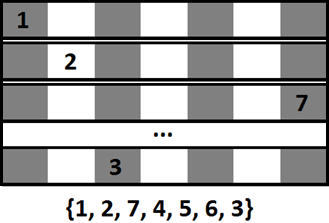
\includegraphics[width=0.35\textwidth]{chromosome.png}
\vspace{-12pt}
\caption{Illustrating the chromosome data structure.}
\label{fig:chromosome}
\end{figure}

\subsubsection{Fitness Function}
Fitness is evaluated by determining the number of collisions between queens on the chessboard - when at least two queens can attack each other, a collision occurs for each queen. This means that in a board state where one queen can attack another, two collisions result. Because it is impossible for there to be more than one queen per column given the chromosome's encoded data structure, only collisions across rows and diagonals must be calculated to determine fitness. The algorithm for determining the fitness of a given board state is given in Algorithm \ref{alg:fitness}, showing the mechanisms we used to find collisions across rows and diagonals. The overall board state fitness is calculated as $fitness = \frac{1}{C}$, where $fitness = 1$ if $C = 0$. The number of collisions is $C$. Maximum fitness is achieved when $C = 0$ as there are no collisions, resulting in a unique board solution. The length of the chromosome corresponds to the number of queens and rows on the square chessboard, $N$. As a result, the fitness function must check across $N - K$ rows and diagonals for each queen, where $K$ is the column index of the current queen.
 

\begin{algorithm}[t!]
  \SetKwProg{Fn}{Function}{}{end}\SetKwFunction{Fitness}{Fitness}%
  \SetKwData{Collisions}{collisions}\SetKwData{Length}{length}\SetKwArray{Chromosome}{$chromosome$}\SetKwData{Yi}{$y_i$}\SetKwData{Yj}{$y_j$}
  \SetKwFunction{Abs}{abs}
  \SetKwInOut{Input}{input}\SetKwInOut{Output}{output}
  \SetAlgoLined
  \DontPrintSemicolon
  
  \Fn{\Fitness{$chromosome$}}
  {
    \Input{A single $chromosome$}
    \Output{A fitness value for the chromosome}
    \BlankLine
    
    \Collisions $\leftarrow$ 0\;
    \Length $\leftarrow$ length of the $chromosome$\;
    \BlankLine
    
    \For{$i \leftarrow 0$ \KwTo $\Length -1$}
    {
      \tcp{Check each gene against the current}
      $j \leftarrow \left( i + 1 \right) \mod{\Length}$\;
      \While{$j$ != $i$}
      {
        \Yi $\leftarrow \Chromosome{i}$\;
        \Yj $\leftarrow \Chromosome{j}$\;
        \BlankLine
        
        \tcp{Check for vertical collision}
        \If{\Yi == \Yj}
        {
          \Collisions $\leftarrow \Collisions + 1$\; 
        }
        \BlankLine
        
        \tcp{Check for diagonal collision}
        \If{\Abs{$\left(i - j \right)$ / $\left(\Yi - \Yj \right)$} == 1}
        {
          \Collisions $\leftarrow \Collisions + 1$\;
        }
        \BlankLine
        
        $j \leftarrow j + 1$\;
        $j \leftarrow j \mod{\Length}$\;
      }
    }
    \BlankLine

    \eIf{\Collisions == 0}
    {
      \KwRet{1}\;
    }
    {
      \KwRet{1 / \Collisions}\;
    }
  }
\caption{Fitness function}
\label{alg:fitness}
\end{algorithm}

\subsubsection{Selection Method}
As in traditional GA, roulette wheel selection was used[CITE]. This process works by filling the roulette wheel with fractional parts of a cumulative probability distribution. In our implementation the range of values will lie between 0 and the sum of all the fitness values of each chromosome in a generation.

Each chromosome is given a fraction of the roulette wheel, whose size is equal to the chromosome's fitness divided by the total fitness of all values. A random floating point value is generated between zero and the sum of the total fitness values. This floating point value will lie within one of the intervals representing one of the chromosomes. Whichever interval it falls in is the selected chromosome. The order in which the chromosomes' intervals are placed doesn't matter, as each 'spin' of the roulette wheel is random - the floating point number generated is created based on a uniformly random distribution.

\subsubsection{Chromosome Operations}
As mentioned in section \ref{params}, the crossover rate is set at a fixed 70\%. This means that 30\% of the time, the genes in the child chromosomes will be an exact clone of the parents. The remaining times, a random crossover occurs. This is done using the traditional GA approach by selecting a random index as the bounds for the portion of the chromosome to cross over. All genes to the right of this index (including the index value itself) are swapped between parents to generate offspring. Between the two parents, the first parent's values to the right of the index, and the second parent's values to the left of the index are combined to create one child (and \textit{vice-versa} for the second child).

Background mutation affects chromosomes randomly after all crossover operations take place. Each next-generation chromosome has a percentage chance of being affected by mutation, and this likelihood changes every generation due to the adaptive variable mutation rate. When a chromosome is selected for mutation, one of the genes in the chromosome is selected randomly. It is then set to a random valid integer. Valid values are between 0 and N corresponding to the index of each row on the chessboard.

% How we evaluate chromosomes in the population and determine distinct solutions
% and apply rotate and reflection to find additional solutions
% The use of terminology here is important DISTINCT implies that the particular
% arrangment of queens is different from another rotation/reflection of the same original
% solution. UNIQUE would consider all reflections/rotations as ONE "unique" solution
\subsubsection{Chromosome Evaluation}
Each generation, there is a likelihood that some of the chromosomes in the current population are valid solutions - any of the current generation's chromosomes with a fitness of 1 is some sort of solution. Whether it is unique or not is unknown at this stage. When a solution is found, it must be compared to the list of previously found solutions to ensure it is not a duplicate. Due to the stochastic nature of the algorithm, there is always a strong possibility that many solutions generated are duplicates of previously found solutions. The symmetry operations applied to each solution found may further increase the likelihood that the new population's solutions that have already been found. Duplicate solutions are discarded without having symmetry operations applied as they would already be identical to symmetric configurations of previously found solutions.

Upon saving any newly found solutions, the new generation replaces the previous generation and the genetic algorithm process cycle continues again.

\subsection{Experimental Methodology}
Experiments were conducted using the high performance computing facilities provided by SHARCNET. Testing of our process was performed by using two different configurations for each N value of the N-Queens problem. Tests were performed for $N = 8, 9, 10$ and so on up to 16, and then at increasing increments of 2 from 18 to 20, 22, 24, 26 and 32. A fixed number of generations was allowed for each trial in order to ensure that the tests had a finite and equal running time. For all runs, 10 million generations were allowed, except for $N = 32$, where 50 million generations were allowed given the increased complexity of the problem.

The first configuration used static mutation rates set at $m = 1\%, 5\%, 10\%$, and every further increment of 5\% up to 100\%. These were used as a control. The second configuration used the adaptive variable mutation rate, and the results were compared. 

For $N = 8$ through 16, 30 tests were performed at each static mutation rate ($21 \times 30 = 630$ tests total), and then 30 runs were performed using variable mutation rates. 

For $N = 18$ through 26, 15 tests were performed under both configurations. For $N = 32$, 10 tests were performed. The decrease in the number of tests performed for higher values of N was largely due to the running time required to generate meaningful results. SHARCNET provisioned us to execute a maximum of 256 jobs at one time, with 7 days CPU time each. The 32-Queens problem required this limit to be fully utilized in order to give results. Given the intractable size of the higher-order N-Queens problems beyond 32-Queens, an unsustainable amount of time and CPU power would be required to finish these problems within our time constraints and were not tested.

Given the volume of data generated by the number of trials, statistical attributes of the results collected (such as mean population fitness and chromosome similarity) were calculated using the mean of every 1000 generations in order to observe the central tendency. A total of roughly 6 gigabytes of data was generated as a result of this process. This was manageable given our allocation of storage space on SHARCNET. The requirements for collecting the data at every generation would have been 1000 times that volume (approximately 6 terabytes) which far exceeded our allocation.

%%%%%%%%%%%%%%%%%%%%%%%%%%%%%%%%%%%%%%%%%%%%%%%%%%%%%%%%%%%%%%%%%
% 
% RESULTS
%
%%%%%%%%%%%%%%%%%%%%%%%%%%%%%%%%%%%%%%%%%%%%%%%%%%%%%%%%%%%%%%%%%
\newpage
\section{Results and Analysis}
It became clear very quickly when we plotted the results of our tests that the variable mutation method was not suitable in its current configuration for the simpler N-Queens problems. In fact, we found that given sufficient knowledge about the problem landscape for the lower-order problems, the right static mutation value would likely beat variable mutation every time. However, for ordinary non-benchmark usage of genetic algorithms it is useless to use a static mutation rate value unless you already know the best mutation rate for the problem. This generally speaks to the point that having an adaptive mutation rate approach will likely find this value. The smaller N-Queens problems are too small to merit the usage of a stochastic approach regardless, as deterministic methods can yield solutions quickly with guaranteed success.

\subsection{'Traversing' the Problem Landscape}
Moving into more complex and larger problems is where the adaptive mutation approach becomes increasingly successful. Our reasoning is that this may have something to do with the similarity threshold value that was chosen (15\%). Further tuning of this parameter may yield better results for larger or smaller problems. We have created a conceptual model for our findings which may yet be validated in future studies.

Mapping the stochastic solution landscape for the N-Queens problem means plotting a random non-deterministic traversal of the solution space to a linear axis. Each sequential value on this axis corresponds to each integer sequence of solutions encoded in the chromosomes. A linear traversal of this landscape implies a uniformly random traversal of the randomly generated solutions. This plot, in contrast to the deterministic solution space yielded by consecutively plotting the values of the integer encoded chromosome, shows very few similarities. There is no way to plot a random traversal except by noting that as time approaches infinity, all solutions will have been traversed and the full contour of the landscape will be visible. This could just as easily be yielded by a consecutive linear traversal, but the point of using GA rather than a deterministic traversal is that GA makes the traversal 'smarter' by searching for values which have better fitness, attracted toward fitness peaks[Genetic Algorithms: a survey]. The mutation operator helps to prevent the current position in the traversal from being stuck in a local optimum[Some improvements on adaptive genetic algorithms for reliability-related applications]. It provides an extra impulse to shift position further towards what a potential solution, and away from previously traversed areas of the landscape.

Given this knowledge, assuming a linear traversal of this random axis is possible in one given test, we can evaluate the characteristics of each GA mutation parameter configuration and map them to this conceptual model. The starting point on the plot is a random location on the landscape. From there, the next location is likely to be within a radius of probable new chromosomes surrounding this area. We have come to refer to this radius of probable chromosomes as the 'step size', and we believe there is some relationship between the step size and the fixed mutation rate. The fixed mutation rate governs the maximum distance from the current position in the traversal to the furthest step away. What this means for a solution landscape like that of the N-Queens problem is that all solutions which are close to the intersections of these steps are easier to find because there is a greater total probability of landing within their vicinity. Solutions which are clustered very close together on this random landscape, however, will likely be stepped around for several generations before convergence on the actual solution occurs.

The variable mutation rate's adaptive nature allows for this fixed step size to be ignored because it introduces the ability to vary the step size when convergence upon a solution occurs. The result is that the probability distribution over the entire solution landscape is more uniformly smaller away from solutions, and larger within the vicinity of solutions. Our reasoning is that if the static mutation rates have a fixed step size, the variable mutation rate does not, and adaptation will vary the step size so as to maintain the chromosome similarity. Further, this decreases the likelihood of overshooting a solution and having to step back around again, because the variability of the mutation rate allows for smaller or larger steps when needed.

In general, this conceptual model will require extensive further study to validate it's correctness. Meanwhile, the empirical evidence presented in our plotted results shows the validity of our adaptive mutation approach.

\subsection{Plotted Results and Observations}
Figure \ref{fig:best_solution_all_queens} depicts the best fixed mutation rate, that found the most solutions for each problem size, versus the variable mutation rate. Each of these plots are cut off at 10 million generations. In spite of the fact that the 32-Queens problem was allowed to run up to 50 million generations, we are only showing plots which are trimmed to this value for consistency of comparison. The plots show that as the problem size increases from the smaller problems up to 14 queens, the fixed mutation rates reach peak performance. In these problems, the most optimal fixed mutation rate is better than the variable mutation rate. This trend changes at the 15 queens where they are nearly equal. From there on, the difference in performance becomes significant - variable mutation consistently finds more solutions than the most optimal fixed mutation rate. 

The optimal fixed mutation rate decrease from 95\% for 8 queens down to 65\% for 32 queens. As the problem size increases, we observe that this trend continues. This can be seen in Table \ref{table:bestsol}. From 15 queens up to 32 queens, there is a divergence between the performance of fixed mutation and variable mutation. A steep decline is visible in the performance of the best fixed mutation rates as the problem size increases. The performance of the variable mutation rate also decreases with increased problem sizes, but at a far lesser rate. This marginal decrease in performance yields the conclusion that variable adaptive mutation rates will perform far better for larger problems.

An interesting result was observed when viewing the box plots showing the range of chromosome similarity values for each static mutation rate. We found that whenever the similarity has the greatest inter-quartile range (IQR), the corresponding static mutation rate performed best. This contributed heavily to the step size concept we believe is exhibited by the system. We also found that as the problem landscape grows larger in higher order N-Queens problems, the IQR decreases in size. There is a possibility that the IQR will decrease towards convergence on a single value in higher order problems, which suggests that there may be a pattern to the convergence which can be approximated and leveraged for predicting optimal static mutation rates for any N-Queens problem. In the 14-Queens problem, the IQR was approximately 20\%. In the 32-Queens problem, the IQR was approximately 3\%. Since testing this requires exhaustive experimentation in order to definitively find the optimal static mutation rate for any given problem, this further supports the notion that a variable mutation rate is a more practical approach. As shown prominently in Figure \ref{fig:fitness_all_mutation_14.png}, we have found that the relationship between the best fixed mutation rates and the largest IQR is visible. The fixed mutation rate of 80\% clearly has the largest IQR, and correspodingly the most number of solutions found. This trend is visible for all values of N in the N-Queens problem. 

However, when approaching problem sizes of $N > 14$, the observation no longer holds true - adaptive variable mutation rates are consistently better, but have comparatively similar IQR to the worse performing static mutation rates. We noticed a new relationship here, showing that the IQR of the variable mutation rate is closest to the trend followed by the IQR of the increasing static mutation rates. There is a sharp drop-off, however, immediately upon reaching the best static mutation rates within this trend. This supports the step-size concept in that we can see the inability of the static mutation rate to converge upon the most desirable fitness values. There is a clear convergence on this value with the adaptive mutation rate, consistently approaching the 25\% fitness value. The most optimal static mutation rate in our experimentation is higher than the true optimum, resulting in a sharp falloff of fitness values. In \ref{fig:best_solution_all_queens}, the 14-Queens problem shows the best static mutation rate is 80\%, which performs substantially better than any other static mutation rate. In Figure \ref{fig:fitness_all_mutation_14.png}, this static mutation clearly has the largest IQR. In the 32-Queens problem, the 65\% fixed mutation rate is the best performer, but is beaten nearly tenfold in performance by the variable mutation rate.

Figure \ref{fig:mutation_rate_all_queens.png} shows a box plot with an overlaid trend line. The box plots in this figure show the IQR for the mutation rate of the variable adaptive method. The points show the best performing static mutation rate for each N-Queens problem. This plot shows the convergence trend of the IQR in the variable mutation rates as the problem size increases. There is also a trend that shows the best performing static mutation rates decrease as the problem size increases. Where the trend and the box plots intersect at the 15-Queens problem, we can see in the corresponding Figure \ref{fig:best_solution_all_queens} that the performance is nearly the same.


\subsection{Why Not Fixed Mutation?}
Variable adaptive mutation gives a distinct advantage over traditional genetic algorithms because of the optimization of a specific parameter [CITE]. By using a variable mutation rate, replacing the mutation parameter with a chromosome similarity, better results can be gleaned while knowing less about the problem landscape or the best static mutation rate to use. Our results show that our variable adaptive mutation approach can perform better than static mutation values for large problems. As the problem becomes too large and unmanageable for traditional deterministic methods, our methodology can still produce useful results. When examining larger problems, our results show that having \emph{a priori} knowledge about the best static mutation parameter still does not yield results as good as those generated from our adaptive mutation approach.

%%%%%%%%%%%%%%%%%%%%%%%%%%%%%%%%%%%%%%%%%%%%%%%%%%%%%%%%%%%%%%%%%
% 
% CONCLUSIONS
%
%%%%%%%%%%%%%%%%%%%%%%%%%%%%%%%%%%%%%%%%%%%%%%%%%%%%%%%%%%%%%%%%%
\section{Conclusions and Further Study}
We conclude that using our variable adaptive mutation rate approach yields better results than traditional GA using fixed mutation rates in larger problems. Further research into adjusting the simplified chromosome similarity parameter that replaces mutation rate may yield even better results. Fixed values were used for our chromosome similarity parameter, and varying this parameter may yield more information about how variable adaptive mutation using our approach can be tuned further towards different problem landscapes.

Exploring our variable mutation rate approach in other NP-Complete combinatorial and optimization problems such as the Traveling Salesman Problem or Constraint Satisfaction Problem may show that our approach is valid for a multitude of problems. We conjecture that this is likely since other adaptive mutation methodologies have yielded performance improvements in various problem domains.

Conducting a multivariate analysis and sensitivity analysis of tuning other parameters in conjunction with the variable adaptive mutation rate may yield further performance improvements. For example, variable population size based on the amount of inbreeding may yield different results. This conjecture is based on the fact that with higher mutation rates, survival fitness decreases, resulting in population shrinkage. Coupling the population size with the mutation rate and patterns of fitness in the GA population may yield a new avenue for future study.

\begin{flushleft}\end{flushleft}

\section{Acknowledgments}
We would like to acknowledge the invaluable contribution made by our supervisor Dr. Shahryar Rahnamayan in transforming a curious junior year artificial intelligence project into a potentially very fruitful course of research. His advice and guidance in shaping our methodology has proved to be crucial to the successful implementation of our experiments.

We would also like to thank the SHARCNET organization for graciously providing the high performance computing facilities we needed to run our experiments.


% The following two commands are all you need in the
% initial runs of your .tex file to
% produce the bibliography for the citations in your paper.
\bibliographystyle{abbrv}
\bibliography{sigproc}  % sigproc.bib is the name of the Bibliography in this case
% You must have a proper ".bib" file
%  and remember to run:
% latex bibtex latex latex
% to resolve all references
%
% ACM needs 'a single self-contained file'!
%

%APPENDICES are optional
%\balancecolumns

%Appendix A
\appendix
\section{Tables}
\begin{table}[!h]
\centering
\caption{Number of unique solutions to the N-Queens Problem}
\begin{tabular}{|l|l|} \hline
N & Distinct Solutions      \\ \hline
1  & 1                      \\
2  & 0                      \\
3  & 0                      \\
4  & 2                      \\
5  & 10                     \\
6  & 4                      \\
7  & 40                     \\
8  & 92                     \\
9  & 352                    \\
10 & 724                    \\
11 & 2680                   \\
12 & 14,200                 \\
13 & 73,712                 \\
14 & 365,596                \\
15 & 2,279,184              \\
16 & 14,772,512             \\
17 & 95,815,104             \\
18 & 666,090,624            \\
19 & 4,968,057,848          \\
20 & 39,029,188,884         \\
21 & 314,666,222,712        \\
22 & 2,691,008,701,644      \\
23 & 24,233,937,684,440     \\
24 & 227,514,171,973,736    \\
25 & 2,207,893,435,808,352  \\
26 & 22,317,699,616,364,044 \\
27 & Unknown				\\
\dots & Unknown				\\
\hline\end{tabular}
\label{table:numuniquesol}
\end{table}

\begin{table*}
\centering
\caption{Best Solution Comparison Between Fixed and Variable Mutation Rates}
\begin{tabular}{|l|l|l|l|l|l|l|} \hline
Queens&               Mutation Rate&  Unique Solutions&   N&      Min Generations&    Mean Generations&   Max Generations\\ \hline
\multirow{2}{*}{8}&   0.95&           92&                 30&     1,793&              4,746&              10,815\\
&                     variable&       92&                 30&     51,23&              15,293&             42,002\\ \hline
\multirow{2}{*}{9}&   0.95&           352&                30&     48,811&             144,456&            372,281\\
&                     variable&       352&                30&     229,242&            1,246,215&          3,038,980\\ \hline
\multirow{2}{*}{10}&  0.9&            724&                30&     188,372&            408,402&            771,208\\
&                     variable&       724&                30&     531,588&            1,629,893&          6,195,099\\ \hline
\multirow{2}{*}{11}&  0.85&           2,680&              30&     2,400,188&          3,799,795&          5,933,213\\
&                     variable&       2,680&              5&      6,900,512&          7,909,269&          9,449,545\\ \hline
\multirow{2}{*}{12}&  0.85&           13,690&             1&      9,890,455&          9,890,455&          9,890,455\\
&                     variable&       11,986&             1&      9,973,787&          9,973,787&          9,973,787\\ \hline
\multirow{2}{*}{13}&  0.8&            32,128&             1&      9,998,058&          9,998,058&          9,998,058\\
&                     variable&       26,308&             1&      9,978,215&          9,978,215&          9,978,215\\ \hline
\multirow{2}{*}{14}&  0.8&            41,520&             1&      9,996,747&          9,996,747&          9,996,747\\
&                     variable&       29,520&             1&      9,999,583&          9,999,583&          9,999,583\\ \hline
\multirow{2}{*}{15}&  0.8&            30,356&             1&      9,982,638&          9,982,638&          9,982,638\\
&                     variable&       30,324&             1&      9,996,584&          9,996,584&          9,996,584\\ \hline
\multirow{2}{*}{16}&  0.8&            15,016&             1&      9,987,788&          9,987,788&          9,987,788\\
&                     variable&       30,132&             1&      9,992,266&          9,992,266&          9,992,266\\ \hline
\multirow{2}{*}{18}&  0.75&           16,392&             1&      9,997,986&          9,997,986&          9,997,986\\
&                     variable&       27,120&             1&      9,998,858&          9,998,858&          9,998,858\\ \hline
\multirow{2}{*}{20}&  0.75&           7,872&              1&      9,972,915&          9,972,915&          9,972,915\\
&                     variable&       25,608&             1&      9,931,631&          9,931,631&          9,931,631\\ \hline
\multirow{2}{*}{22}&  0.7&            6,008&              1&      9,959,712&          9,959,712&          9,959,712\\
&                     variable&       25,376&             1&      9,991,089&          9,991,089&          9,991,089\\ \hline
\multirow{2}{*}{24}&  0.7&            6,440&              1&      9,929,626&          9,929,626&          9,929,626\\
&                     variable&       24,560&             1&      9,998,508&          9,998,508&          9,998,508\\ \hline
\multirow{2}{*}{26}&  0.7&            6,280&              1&      9,969,840&          9,969,840&          9,969,840\\
&                     variable&       23,008&             1&      9,983,128&          9,983,128&          9,983,128\\ \hline
\multirow{2}{*}{32}&  0.65&           15,216&             1&      49,732,320&         49,732,320&         49,732,320\\
&                     variable&       104,080&            1&      49,996,701&         49,996,701&         49,996,701\\
\hline\end{tabular}
\label{table:bestsol}
\end{table*}


\section{Figures}
\begin{figure}[h]
\centering
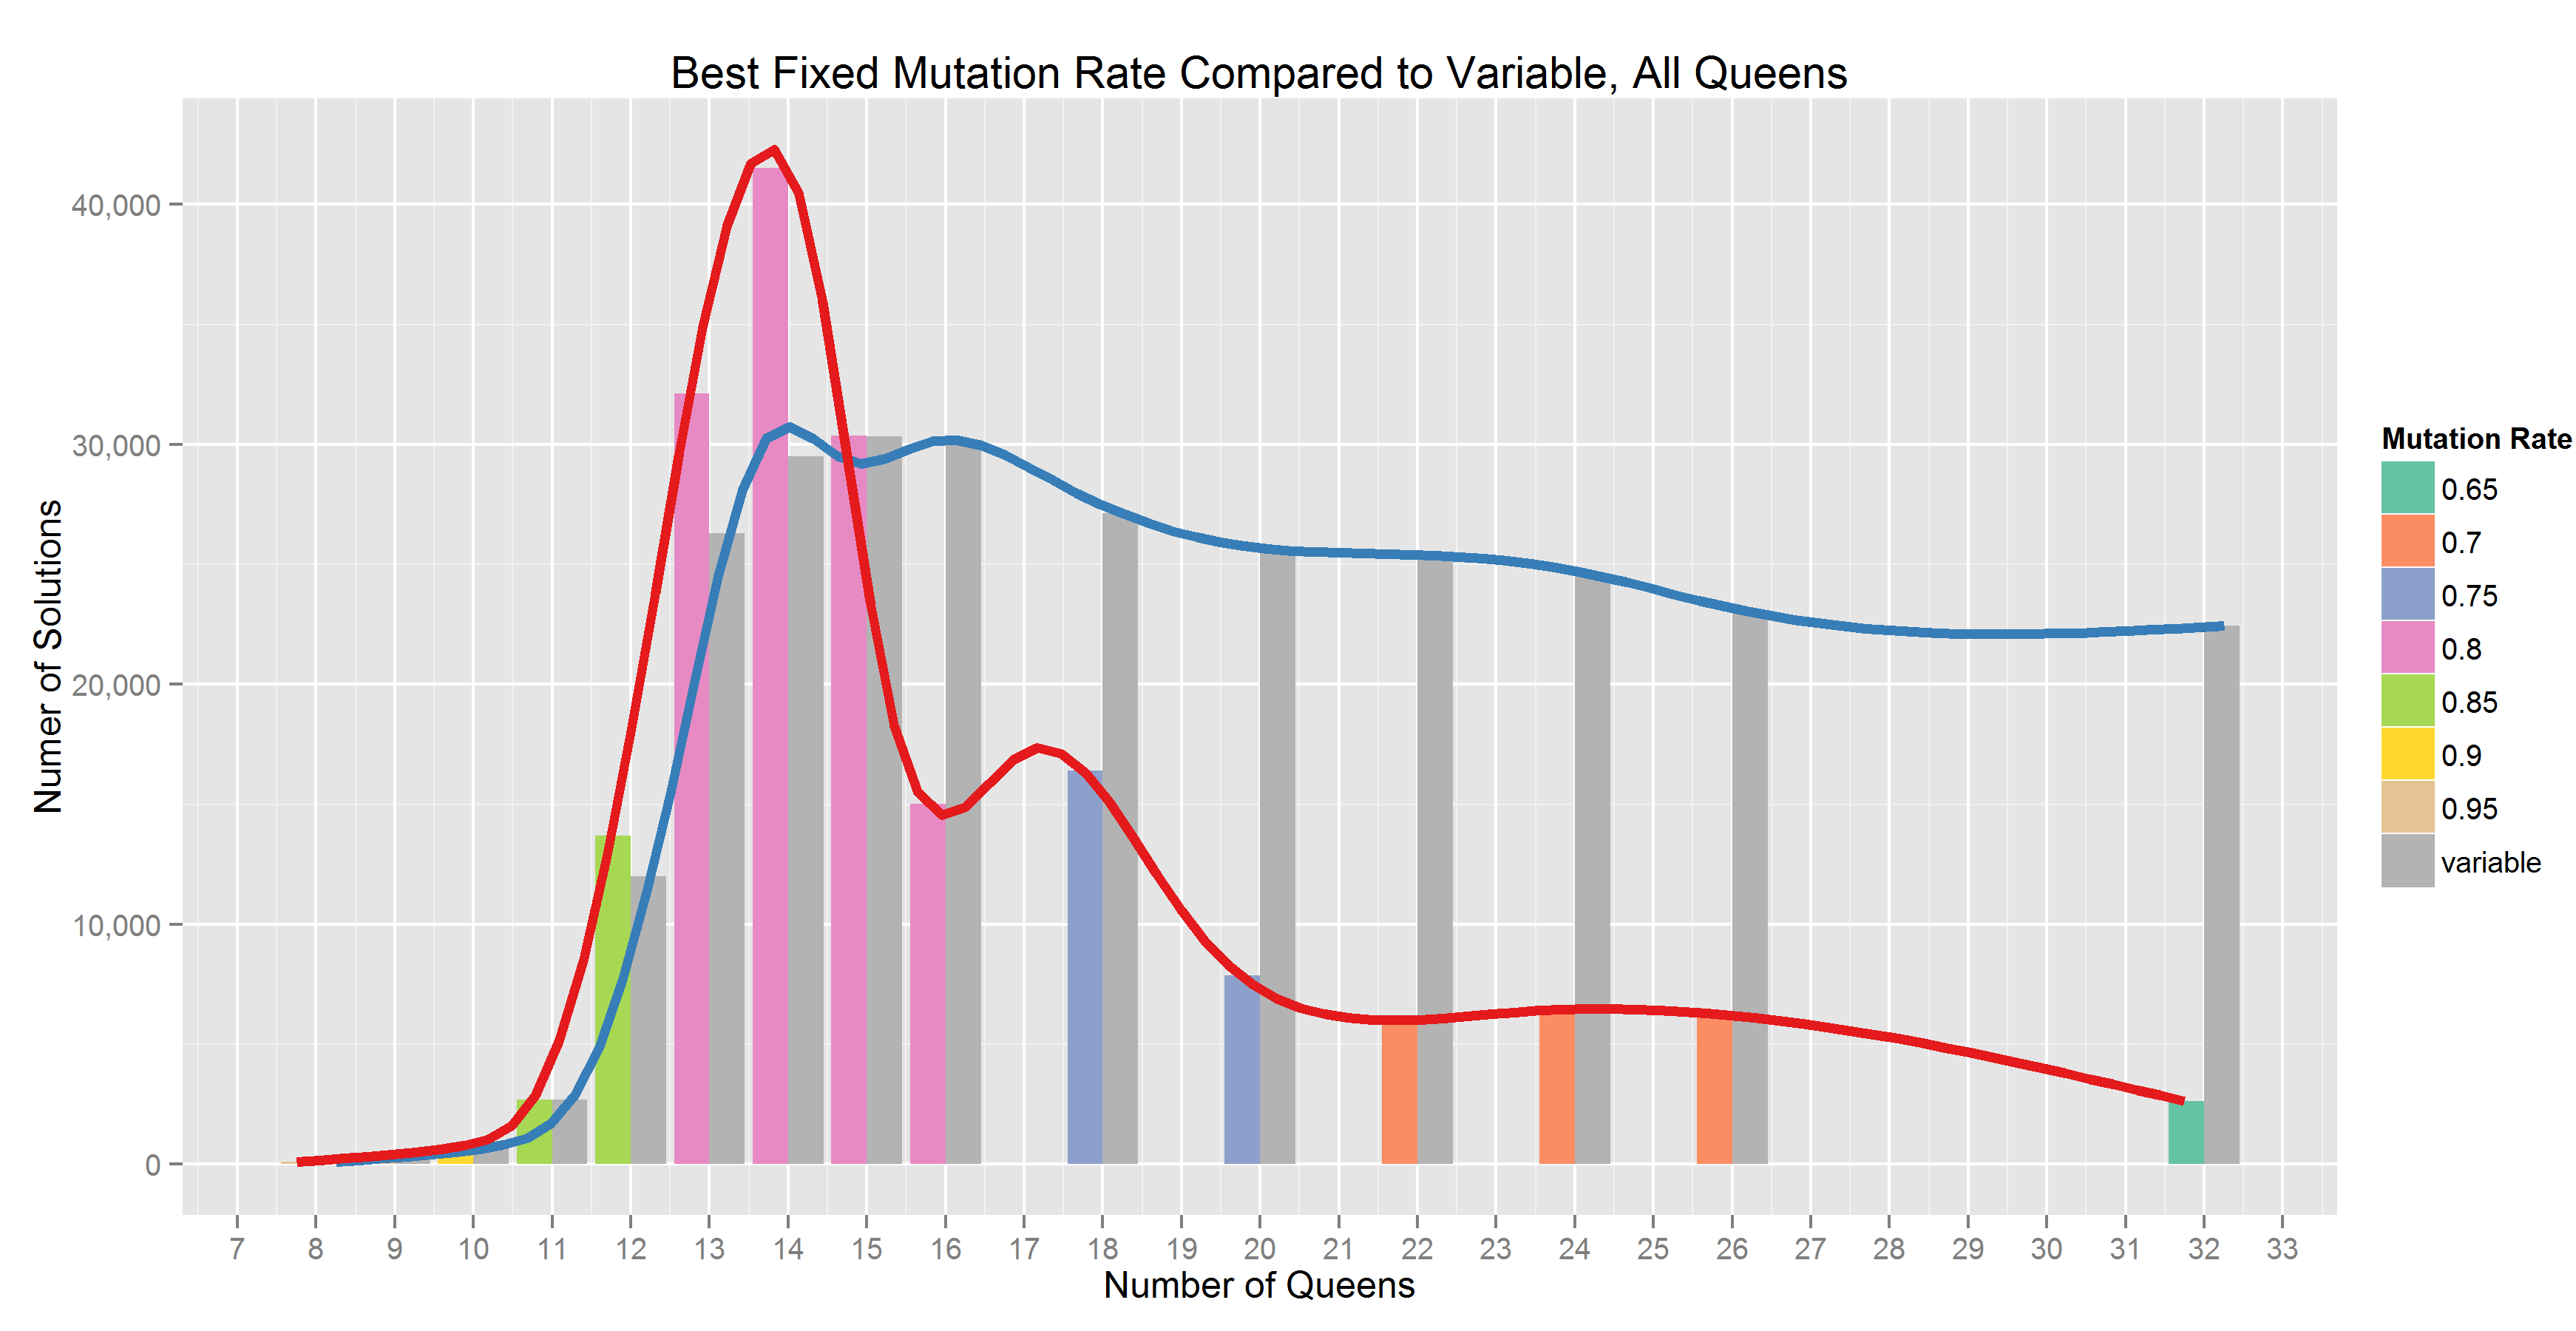
\includegraphics[width=0.35\textwidth]{best_solution_all_queens.png}
\vspace{-12pt}
\caption{}
\label{fig:best_solution_all_queens}
\end{figure}

\begin{figure}[h]
\centering
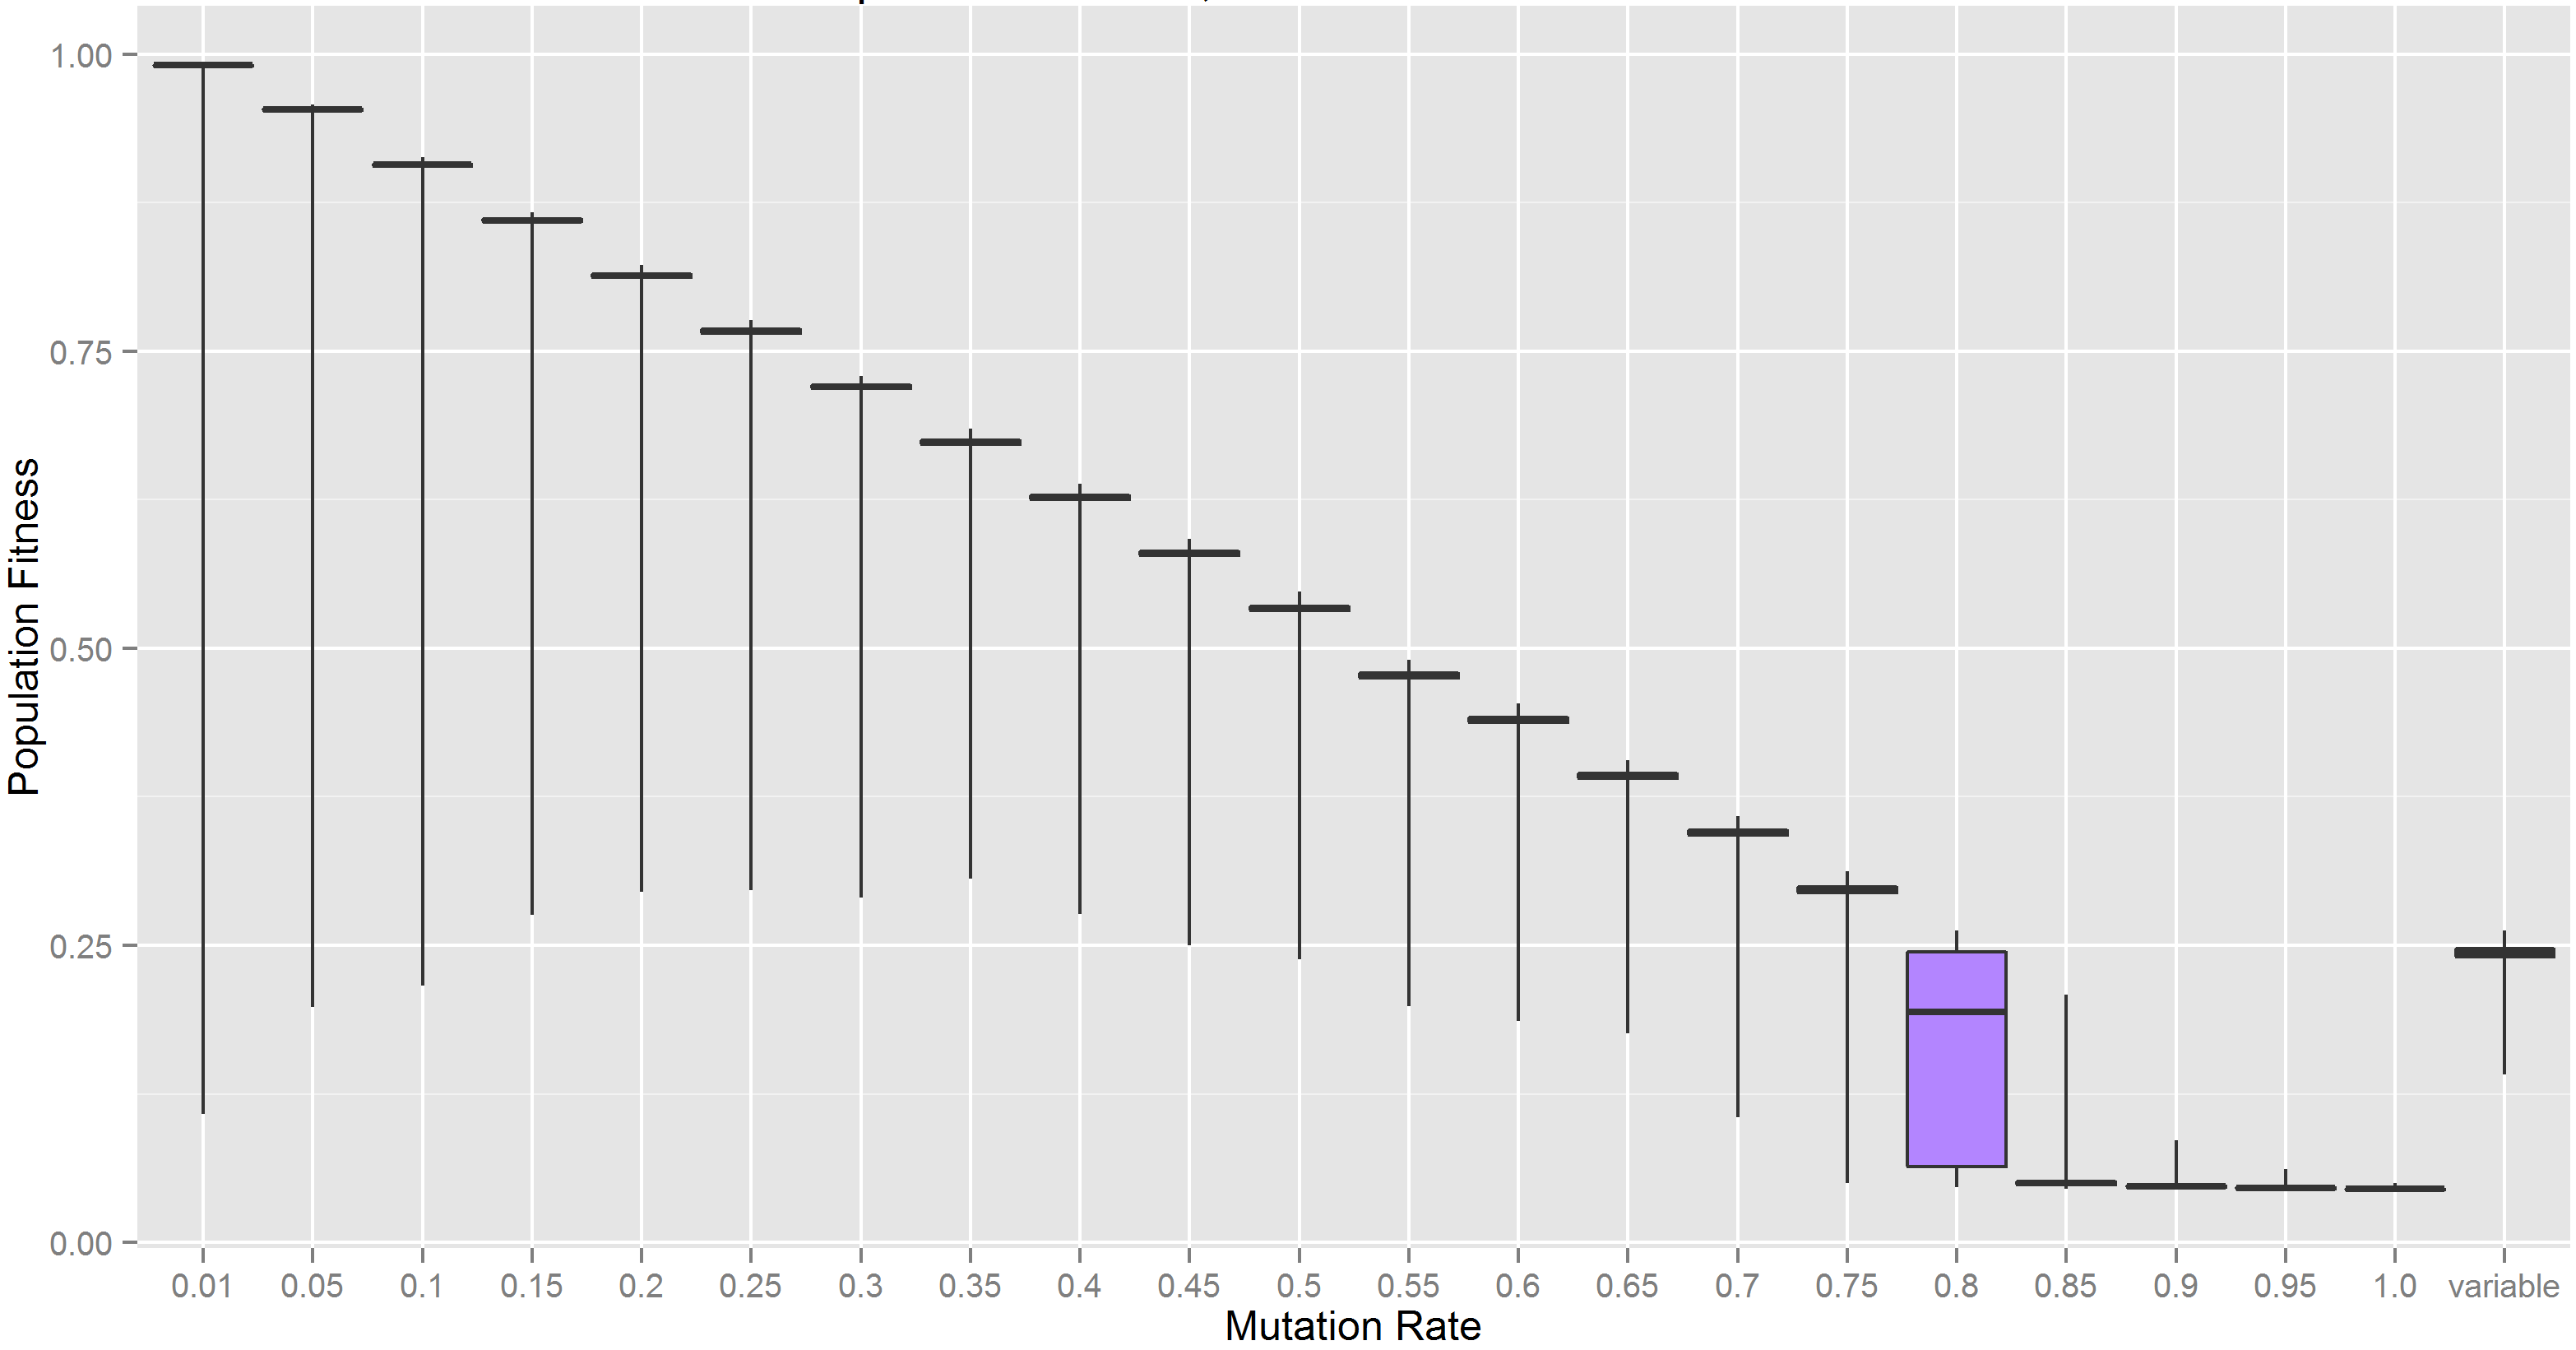
\includegraphics[width=0.35\textwidth]{fitness_all_mutation_14q.png}
\vspace{-12pt}
\caption{}
\label{fig:fitness_all_mutation_14}
\end{figure}


\begin{figure}[h]
\centering
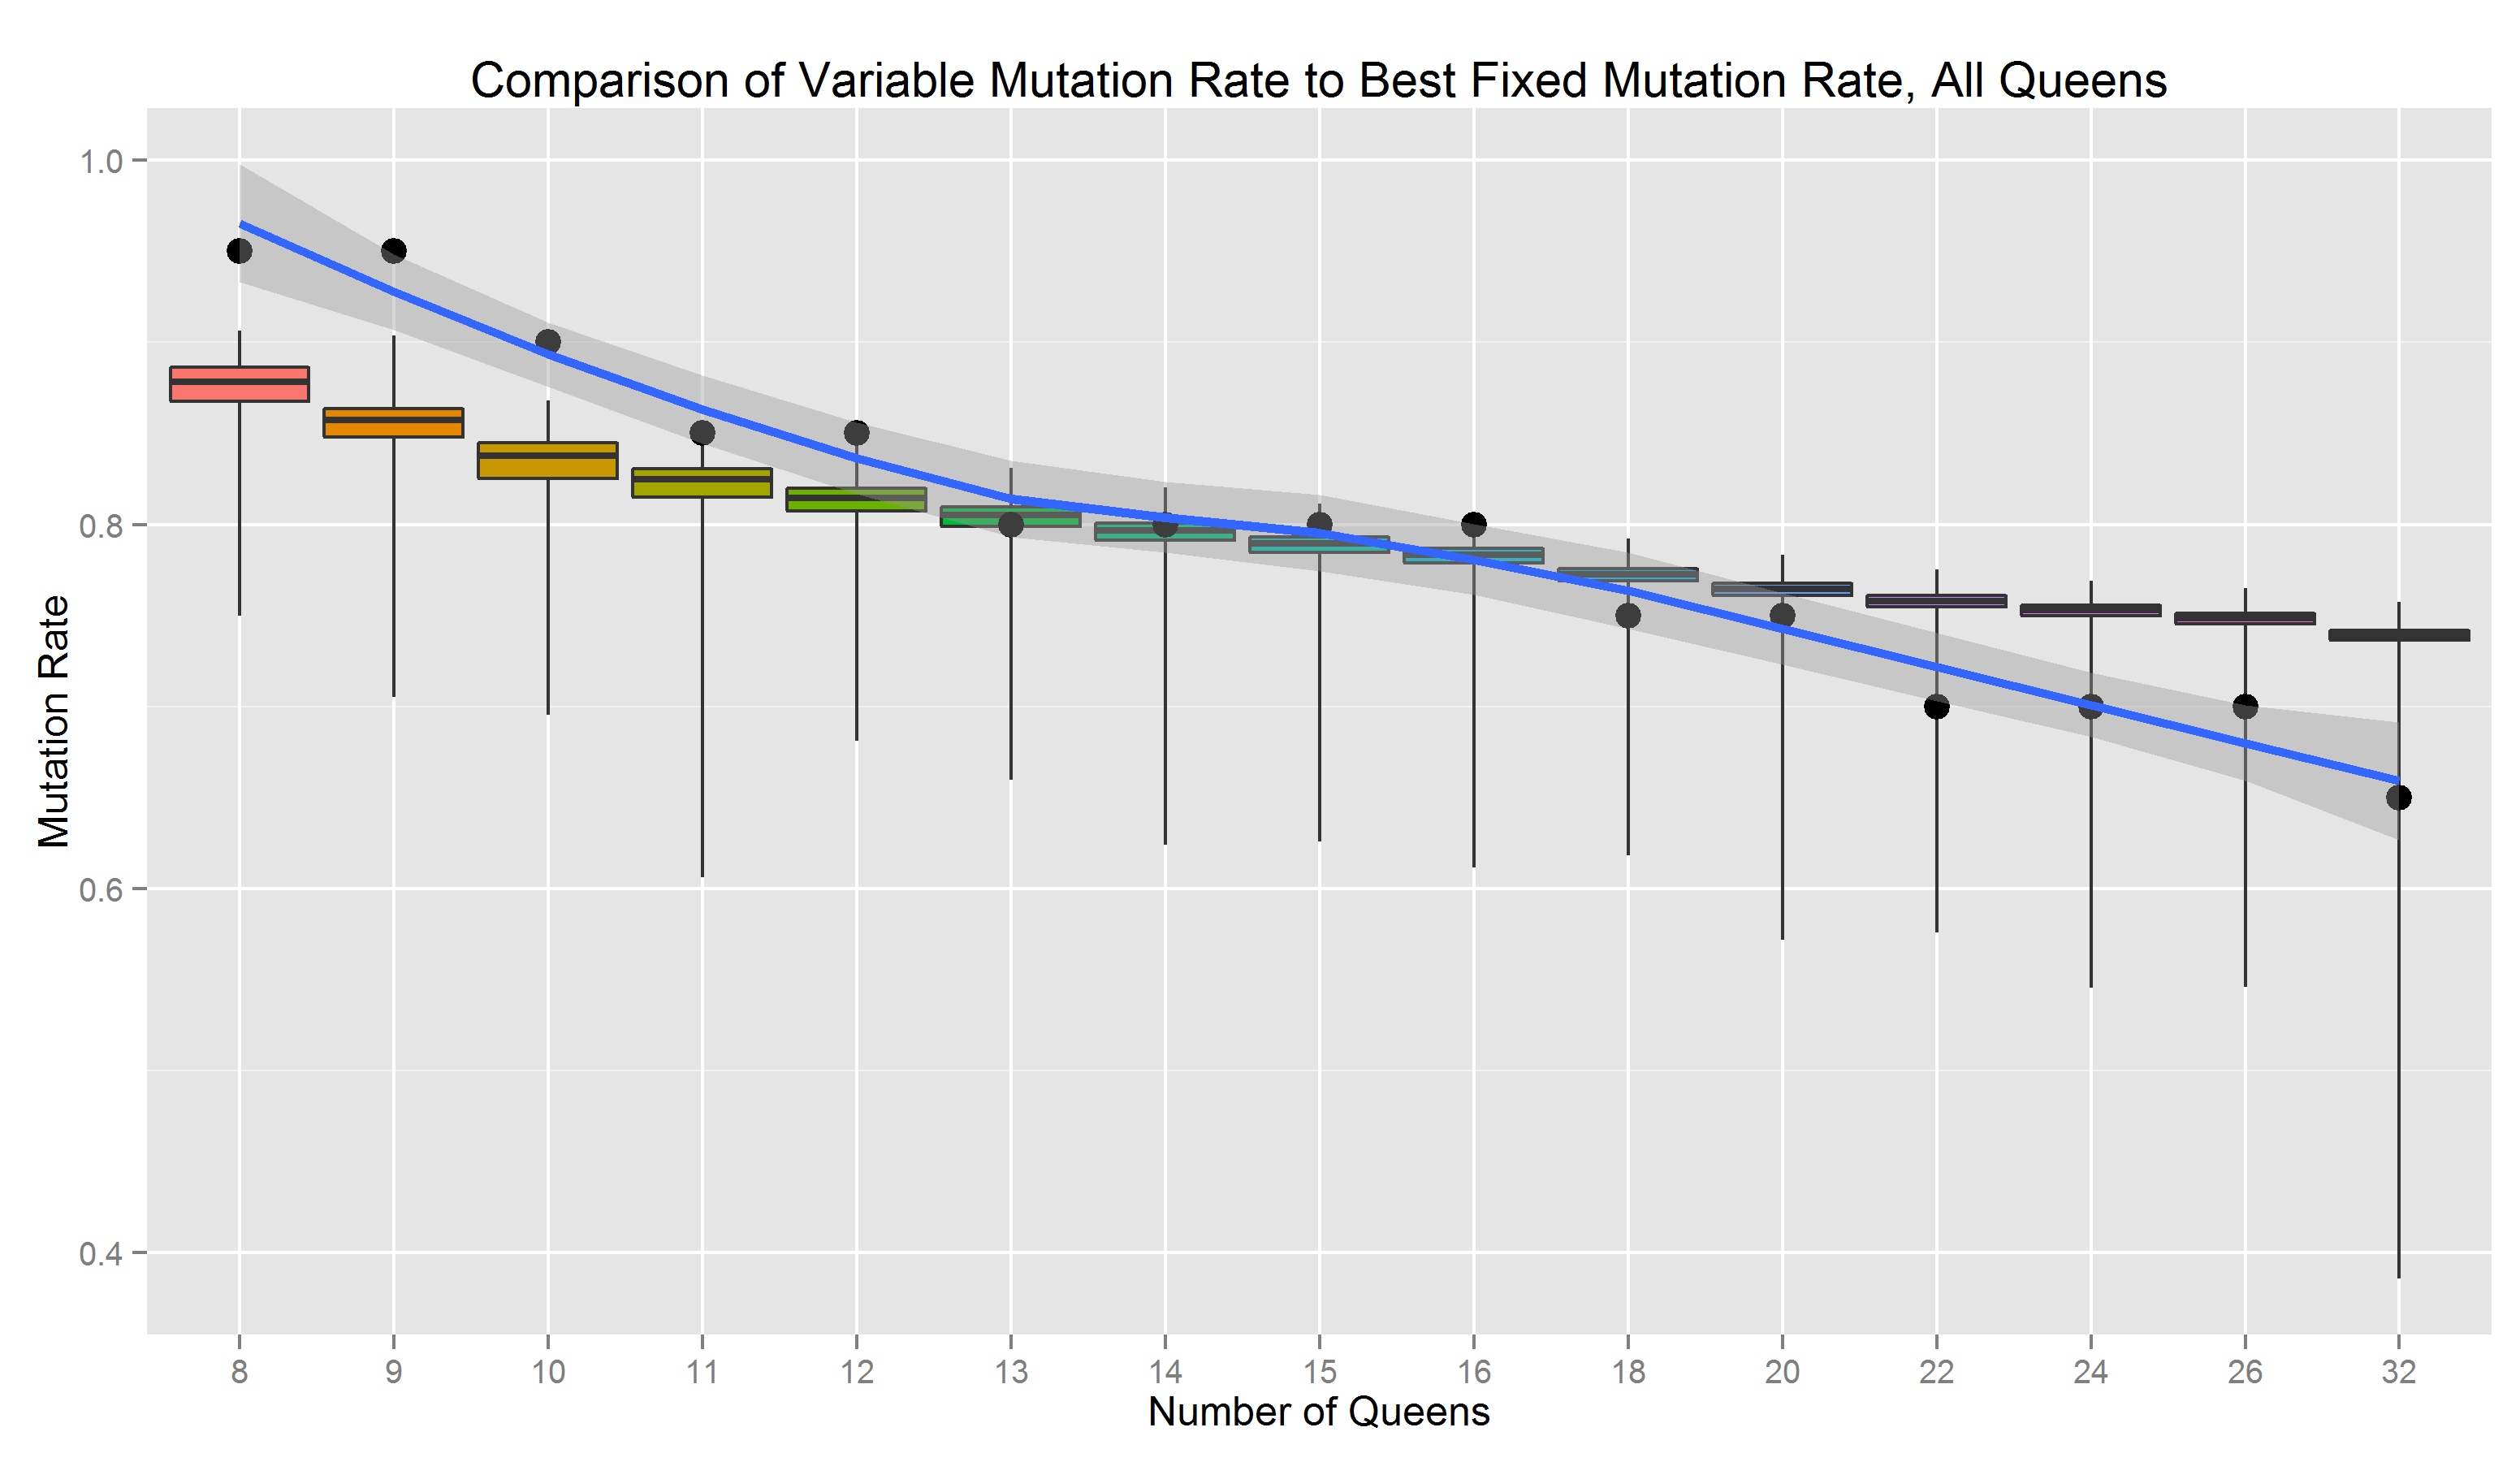
\includegraphics[width=0.35\textwidth]{mutation_rate_all_queens.png}
\vspace{-12pt}
\caption{}
\label{fig:mutation_rate_all_queens}
\end{figure}

\end{document}
